\documentclass[preprint,times]{elsarticle}
% For a two-column layout close to the published Procedia CIRP page, replace the
% line above with:
%   \documentclass[final,5p,times,twocolumn]{elsarticle}

\usepackage{amsmath,amssymb}
\usepackage{graphicx}
\usepackage{booktabs}
\usepackage{siunitx}
\usepackage{lineno}
\usepackage{array}
\usepackage{tabularx}
\usepackage{rotating}
\usepackage{xurl}
\usepackage{float}
\usepackage{placeins}
\usepackage{tikz}
\usetikzlibrary{arrows.meta,positioning,shapes.geometric,fit}
\usepackage[T1]{fontenc}
\usepackage{xcolor}
\usepackage{hyperref}
\hypersetup{colorlinks=true,linkcolor=blue,citecolor=blue,urlcolor=blue}

\newcolumntype{M}{>{\hsize=1.5\hsize\raggedright\arraybackslash}X}
\newcolumntype{D}{>{\hsize=0.6\hsize\centering\arraybackslash}X}
\newcolumntype{T}{>{\hsize=0.6\hsize\centering\arraybackslash}X}
\newcolumntype{S}{>{\hsize=1.5\hsize\raggedright\arraybackslash}X}
\newcolumntype{F}{>{\hsize=0.8\hsize\raggedright\arraybackslash}X}

\journal{[Journal name -- see cover letter]}

% compact reference list, as in the published Procedia page
\setlength{\bibsep}{0pt plus 0.3ex}

\begin{document}

\begin{frontmatter}

\title{Which process faults can be told apart? Diagnosability limits of
in-situ monitoring in laser powder bed fusion}

%% ---------------------------------------------------------------------------
%% TODO before submission: complete author list, affiliation and corresponding
%% author details. The entry below is a placeholder.
%% ---------------------------------------------------------------------------
\author[a]{Amit Jain\corref{cor1}}
\ead{amitkjain23@gmail.com}
\cortext[cor1]{Corresponding author.}
\affiliation[a]{organization={[Affiliation to be completed]},
                city={[City]},
                country={[Country]}}

\begin{abstract}
In-situ monitoring is standard on metal additive manufacturing systems, and
classifiers report high accuracies for detecting defects from photodiode and
imaging signals. Those results answer a question about outcomes: which defect
formed. Specifying hardware requires an answer one step upstream --- which
process \emph{causes} a sensor configuration can separate in principle, and which
remain confounded whatever classifier is applied. Where two causes produce
signatures differing by less than the sensor noise, no volume of training data
distinguishes them; the limit is structural, not algorithmic. This paper applies
structural and quantitative diagnosability analysis, mature in automotive and
aerospace process control, to laser powder bed fusion. A calibrated
reduced-order thermal model generates the response of a coaxial suite to five
injected faults: laser power and scan speed deviation, thin powder layers from
recoater short-feed, degraded shielding gas flow, and geometry-driven heat
accumulation, with separability measured as an angle between noise-whitened
fault signatures. Laser power and gas degradation prove \emph{exactly} confounded
instantaneously, by algebra rather than noise, so no instrument reading the melt
pool separates them, and seven candidate observables raise the attainable rank
only from three to four. Regressing the same three sensors onto known build
context raises the rank to five and the worst pair from $0.00^\circ$ to
$25.83^\circ$ at no hardware cost, outperforming two idealised direct
measurements of the causes themselves. Diagnosability matrices are reported for
five configuration classes typical of commercial machines.
\end{abstract}

\begin{keyword}
Additive manufacturing \sep Process monitoring \sep Diagnosability \sep
Fault diagnosis \sep Laser powder bed fusion
\end{keyword}

\end{frontmatter}

%% ===========================================================================
\section{Introduction}

Laser powder bed fusion (LPBF) builds a part by melting thousands of short track
segments per layer, and a modest excursion in any of several independent inputs
can produce a rejected part. Machine manufacturers have responded by fitting
in-situ monitoring as standard --- coaxial photodiodes, melt pool cameras,
pyrometers, and increasingly acoustic and powder-bed imaging --- and a large
literature maps those signals onto defects with high reported accuracy.

Almost all of that work answers a question about \emph{outcomes}: given the
signals, which defect formed? That matters for part acceptance, but it is not the
question a machine builder asks when specifying hardware, nor the one a process
engineer asks when a build drifts. Those concern \emph{causes} --- the laser is
under-delivering, the recoater is short-feeding, the gas flow has degraded ---
and which it is determines what gets corrected.

The distinction is not semantic, because causes can be mutually
indistinguishable in a way outcomes are not. If two causes drive the readings
along the same direction in signal space, the readings contain no information
separating them, and no classifier, however trained, can recover the difference.
The limitation is structural --- a property of the measurement and the physics,
not of the algorithm. Conversely, a pair separable in principle but misclassified
in practice is an algorithm that can be improved.

Diagnosability analysis is the established discipline for deciding which case
holds. Developed within model-based fault detection and isolation (FDI), it asks,
before any estimator is built, which faults a given measurement set can detect
and which it can isolate from one another \cite{Krysander2008,Frisk2017}. The
methods are standard where sensor sets are costly and must be justified in
advance, but to the authors' knowledge they have not been applied to LPBF.

This paper applies them. A calibrated reduced-order thermal model is driven by
five injected fault modes, the resulting signatures are compared pairwise against
noise, and the outcome is a diagnosability matrix per configuration, dividing
fault pairs into those resolvable from existing signals, those needing an added
measurement, and those structurally irreducible. The contributions are: what the
authors believe to be the first diagnosability matrix for the process; a
demonstration that laser power and shielding gas degradation are \emph{exactly}
confounded instantaneously, so no melt-pool instrument separates them; the
finding that the binding limit is the melt pool rather than the instrumentation;
and the demonstration that build structure already present dissolves that limit
at no hardware cost, outperforming two idealised direct measurements of the
causes.

\section{Background and related work}

\subsection{What in-situ monitoring classifies}

Melt pool monitoring with coaxial photodiodes and cameras is the most widely
deployed configuration, and its canonical application is flaw classification.
Scime and Beuth identified signatures indicative of keyholing porosity and
balling from high-speed visible imaging \cite{Scime2019}, and later work extended
this across modalities and alloys, including mechanical-property prediction from
coaxial signals \cite{Raj2023}. In each case the predicted
quantity is an outcome or a material state, and whether two distinct excursions
could have produced the same signal is not posed.

A smaller body of work estimates process inputs, and is closer to the present
question. RAISE-LPBF reconstructs laser power and scan speed independently from
on-axis video on 316L, sampling both per scan line from continuous distributions
so interactions can be studied \cite{Blanc2024}. Reijonen reports coaxial
photodiode response to power, speed, focal position, scan orientation and
shielding gas flow, finding power approximately linear, speed a power law, and
the remainder non-linear and interactive \cite{Reijonen2024}. These characterise
\emph{sensitivity}; identifiability --- whether sensitivities to different causes
are linearly distinguishable --- is the question neither addresses.

Sensing that observes the powder bed forms a third class, attacking causes the
melt pool reports only indirectly: Liu et al.\ recover local powder layer
thickness and thermal transport from the post-recoat heat-up transient
\cite{Liu2022}, and Bugatti and Colosimo detect geometric and surface
anomalies below 100\,\textmu m with a recoater-mounted contact image sensor
\cite{Bugatti2022}. Both need added hardware and neither is simulated here; they
appear in Section~\ref{sec:added} as targets, not modelled options.

\subsection{Lumped process metrics are incomplete}

A recurring pattern is to report a \emph{lumped} process quantity in place of its
components. Volumetric energy density (VED) is the usual choice, and
state-of-the-art parameter estimation from melt pool imagery still predicts
energy density \emph{class} rather than power and speed separately
\cite{kNN2025}.

There is direct evidence that this discards information. Guo et al.\ held input
energy density constant while varying power and speed together, and observed melt
pool dimensions and volume changing by orders of magnitude with transitions
between melting regimes, attributing it to the two altering absorption
differently through the vapour depression \cite{Guo2019}. Independently, the 2022 Additive Manufacturing Benchmark found single-track depth
correlated with VED while width did not \cite{Weaver2024}. Falling back on a
lumped group is the natural response to confounded components; whether they are
confounded for a given suite is a diagnosability question, and is what the
literature has not established.

\subsection{Diagnosability analysis}

Model-based diagnosability analysis operates on a model expressed over known
variables, unknown variables and faults. Structural analysis considers only which
variables appear in which equations, discarding numerical values, and determines
detectability and isolability from the resulting bipartite graph; minimal
structurally overdetermined (MSO) sets identify the redundant subsystems from
which consistency tests are built \cite{Krysander2008,Frisk2017}. Being purely combinatorial it scales to large nonlinear models and is
insensitive to parameter error, but it can be optimistic: two faults may be
structurally isolable yet numerically indistinguishable. Quantitative analysis
supplies the remainder, by linearising the fault-to-measurement map and
examining the geometry of the resulting signature directions. This paper runs
both, using the structural result as an independent check.

%% ===========================================================================
\section{Method}
%% ===========================================================================

\subsection{Forward model and calibration}

Melt pool geometry is computed from the Eagar--Tsai solution for a moving
Gaussian heat source on a semi-infinite solid, extended with the
Gladush--Smurov keyhole depth correction following Honarmandi et al.\
\cite{Hon2021}. Four parameters --- effective absorptivity, effective
conductivity, heat capacity and the keyhole constant --- are fitted to the seven
IN718 bare-plate single-track cases of the 2022 Additive Manufacturing Benchmark
\cite{Weaver2024}, giving \textbf{11.7\,\% error on melt pool width and 13.0\,\%
on depth}. The keyhole correction is necessary rather than optional: all seven
cases have depth-to-half-width aspect ratios between 1.45 and 4.28, and pure
conduction gives a 27.8\,\% depth error on the same cases.

The quadrature in the Eagar--Tsai history integral and the derivative step are
both set by convergence tests rather than assumed. Central differences
$[y(+h)-y(-h)]/2h$ are evaluated at $h=0.002$; entries still move by 39.4\,\% between $h=0.04$ and $h=0.02$, fall
below 0.3\,\% at $h=0.005$, and the residual error follows the second-order
scaling the central-difference expansion predicts.

\subsection{Fault definitions}

Five causes are modelled, each defined as a \emph{physical} quantity acting on a
model input so that no arbitrary severity-to-signal constant is introduced. For
fault magnitude $f$: \emph{power} scales laser power, $P(1+f)$; \emph{speed}
scales scan speed, $v(1+f)$; \emph{gas} is a plume optical depth attenuating
effective absorptivity, $A\,e^{-f}$; \emph{geometry} is a preheat rise in units
of 100\,K, $T_0+100f$; and \emph{layer} is a fractional layer-thickness
deviation acting through three channels, below. A positive layer fault denotes a
\emph{thinner} layer, as produced by recoater short-feed.

The layer fault acts through three channels, two derived from published
measurement. Its absorptivity coupling, $-0.230$, follows from the
powder-to-solid absorptivity ratio of approximately two measured
calorimetrically at 1070\,nm \cite{Trapp2017} combined with a radiative
penetration depth of a few particle diameters; it implies a bare-solid
absorptivity of 0.258, consistent with literature values for nickel alloy at
1\,\textmu m and with the fitted value. Its
powder-melting enthalpy coupling, $+0.186$, follows from an energy balance in
which melting the layer consumes 15.7\,\% of the absorbed energy, so a thinner
layer frees proportionally more for substrate penetration. Its conductivity
coupling remains an unmeasured estimate, swept across its plausible range in
Section~\ref{sec:robust} with every conclusion invariant to it. All couplings are applied in exponential form $A\,e^{cf}$, which agrees with
$A(1+cf)$ to first order but cannot pass through zero, where the linear form
would drive thermal diffusivity negative and the Eagar--Tsai integrand
imaginary.

\subsection{Sensor models}

Three coaxial observables are computed from the temperature field: a
band-integrated photodiode (700--1000\,nm), melt pool area, and a two-colour
pyrometer (750/950\,nm) evaluated as the ratio of integrated band powers and
inverted for temperature. Spectral radiance follows Planck's law, with temperature capped at the boiling
point before any radiance is computed. Four further candidate observables are
defined for Section~\ref{sec:melt}: the camera's width and length axes reported
separately, a short-wave infrared photodiode, and a wide-band pyrometer.

\subsection{Diagnosability measures}

The relative-sensitivity Jacobian is
%
\begin{equation}
J_{sk} \;=\; \frac{1}{y_s}\,\frac{\partial y_s}{\partial f_k},
\label{eq:jac}
\end{equation}
%
so entry $(s,k)$ is the fractional change in sensor $s$ per unit of fault $k$,
making rows with different physical units comparable. Each row is divided by that
sensor's relative noise $\sigma_s$ to give the whitened matrix $J^{\mathrm{w}}$.

Three quantities are reported throughout. The \emph{angle} between whitened
columns, $\theta_{kl} = \arccos\big(|\langle J^{\mathrm{w}}_{:k},
J^{\mathrm{w}}_{:l}\rangle| \,/\, \|J^{\mathrm{w}}_{:k}\|
\|J^{\mathrm{w}}_{:l}\|\big)$, measures pairwise separability: $0^\circ$ means the two faults move the readings
along one line and are indistinguishable by any estimator, $90^\circ$ that they
are orthogonal. A practical floor of $10^\circ$ is adopted as a convention and
its influence reported rather than assumed. The \emph{rank} of $J^{\mathrm{w}}$
counts how many fault directions are observable at all, and the \emph{condition
number} --- the ratio of largest to smallest non-zero singular value --- how thin
the weakest is; rank without it is misleading, as Section~\ref{sec:melt} shows.
Structural analysis is run in parallel on an eleven-equation representation of
the same model using MSO sets, as an independent check.

\subsection{Build context and the enlarged observation}
\label{sec:context}

A build is not a single instant. It comprises thousands of segments whose
toolpath, layer index, gas-flow direction and local geometry are known to the
machine, and the five faults do not vary identically across them: laser
degradation drifts with time, galvanometer error concentrates at direction
reversals, a recoater short-feed recurs with layer index, gas degradation follows
the flow direction, and heat accumulation follows support depth. Treat the build,
not the instant, as the observation: let
$G\in\mathbb{R}^{N\times 5}$ hold five known context regressors over $N$
segments --- a constant, position along the gas-flow axis, layer parity, turn
density and support depth --- and $M\in\mathbb{R}^{N\times 5}$ the spatial
modulation profile of each fault. Regressing each sensor's relative residual onto
$G$ yields five coefficients per sensor in place of one reading, so three sensors
give $3\times5=15$ observables, with Jacobian
%
\begin{equation}
J^{\mathrm{big}}_{(s,j),k} = J_{sk}\,B_{jk},
\qquad B = (G^{\!\top}G)^{-1}G^{\!\top}M .
\label{eq:big}
\end{equation}
%
The noise on the $j$-th coefficient from sensor $s$ is not $\sigma_s$ but
$\sigma_{(s,j)} = \sigma_s\sqrt{[(G^{\!\top}G)^{-1}]_{jj}}$, which here lies
between 0.109 and 0.136, so fitting $N=84$ segments to five regressors buys
roughly a ninefold noise reduction. Results use $N=84$; the
dependence on $N$ is given in Section~\ref{sec:robust}.

The profiles in $M$ are physical claims rather than measurements, and one has
direct experimental support. The AM Bench pad scans \cite{Weaver2024}, under a
4.3\,m\,s$^{-1}$ cross-flow, show melt pool depth reduced by 27.2\,\% on average
(range 19.4--31.5\,\% over four cross-sections) on tracks scanned parallel to the
gas flow relative to anti-parallel tracks, against expanded uncertainties of
6--11\,\textmu m on depths near 175\,\textmu m, attributed to vapour-plume
interaction with the laser. The measurement carries its own control: on pads
scanned perpendicular to the flow the odd--even difference is 2.4--4.7\,\%,
within or near uncertainty. A deterministic gas-related modulation of melt pool
geometry, tied to a known toolpath quantity, is therefore established by
measurement rather than asserted.

Two qualifications follow from the same source. The measured modulation is
organised by scan direction relative to the gas flow rather than by position
along it, and it alternates at track scale where a recoater signature alternates
at layer scale --- so the two have distinct periodicities, which
Section~\ref{sec:robust} shows is the condition the method actually requires.

\subsection{Position on sensor noise}

Only one in-process noise figure proved citable: a melt pool width uncertainty of
2.3\,\% relative, from the uncertainty budget of Weaver et al.\
\cite{Weaver2024}. No comparable in-process characterisation was found for a
coaxial photodiode or two-colour pyrometer; published thermal calibration work
for such sensors reports instrument calibration, not in-process noise.
Sensor noise is therefore treated as a \emph{ratio} and swept over four
assumption sets, with every conclusion required to hold under all of them. This
suffices for isolability, which depends only on relative noise --- angles, rank
and condition number are invariant to a common scaling of all sensor noise ---
so absolute detection thresholds are \textbf{not} claimed.

%% ===========================================================================
\section{Results}
%% ===========================================================================

\subsection{Validation}

Two checks are made against data not used in the fit. Over 27 melted conditions
the model reproduces the benchmark correlation structure: depth correlates with
volumetric energy density ($r=+0.727$) while width does not ($r=+0.032$)
\cite{Weaver2024}. Against the constant-energy-density experiment of Guo et al.\
\cite{Guo2019} the model achieves a \textbf{partial pass}: it reproduces the
existence, direction and regime transition of the variation, but spans
2.37$\times$ in depth where the experiment reports orders of magnitude. The
mechanism Guo et al.\ identify --- absorption varying with vapour depression
geometry --- is absent from a conduction solution with an analytic keyhole patch,
and this is reported as a model limitation. The same sweep yields a result used
in Section~\ref{sec:added}: at constant energy density melt pool \emph{length}
varies by 2.53$\times$ while width and depth vary by only 1.11$\times$.

\subsection{Laser power and shielding gas are exactly confounded}

Both faults act \emph{only} on the product (effective absorptivity $\times$
power), and the Eagar--Tsai temperature rise is linear in that product. Choosing
$f_{\mathrm{gas}}=-\ln(1+f_{\mathrm{power}})$ therefore produces an identical
melt pool: the same temperature at every point, hence identical readings from any
instrument that could be built. The ratio of the two Jacobian columns is
$-0.99999$, $-1.00000$, $-0.99993$ across the three sensors, a spread of
$7\times10^{-5}$ attributable to finite-difference error on an exact identity.
The pairwise angle is \textbf{0.00$^\circ$}. This is an algebraic degeneracy, not
a numerical coincidence: sweeping every coupling constant across its plausible
range leaves the angle at $0.00^\circ$, and the independent structural analysis
identifies the same pair from equation form alone.

\subsection{The limit is the melt pool, not the sensor count}
\label{sec:melt}

The whitened $3\times5$ Jacobian has singular values 3.451, 0.155 and 0.041 ---
rank 3, condition number 85 --- so two fault directions are unobservable, and
they are computable. The dominant one is $(\text{power}+0.670,\
\text{gas}+0.731,\ \text{layer}-0.112,\ \text{speed}-0.056)$; applied as a real
fault of 5\,\% vector norm it moves the sensors by $-0.083\,\%$, $-0.067\,\%$ and
$-0.002\,\%$, against $+7.03\,\%$, $+6.02\,\%$ and $+0.049\,\%$ for a plain 5\,\%
power fault --- a factor of 85, the condition number.

Adding all four candidate observables gives seven rows and raises the rank only
from 3 to \textbf{4}. The fourth direction is of no practical use: the singular
values become $(4.58,\ 0.475,\ 0.199,\ 2.0\times10^{-5},\ 3.9\times10^{-6})$, a
condition number of $2.3\times10^{5}$, and the worst pairwise angle remains
$0.00^\circ$. Seven instruments leave power and gas exactly as confounded as one.

The reason is structural. Everything the model knows funnels into four physical
channels --- absorbed power, scan speed, effective conductivity and preheat ---
with three of the five faults crowding onto the first. Any instrument reading
only the melt pool is a function of those four channels, so the fault-to-sensor
map cannot exceed rank 4 however many are fitted: a new wavelength reweights the
same Planck curve over the same pool, adding a row, not a direction.

\subsection{Build context dissolves the limit}

With the enlarged observation of Section~\ref{sec:context}, rank rises from 3 to
\textbf{5}, the worst pair from $0.00^\circ$ to \textbf{25.83$^\circ$}, power
versus gas to $29.34^\circ$, and the condition number falls from 85 to 30. All
ten pairs clear the $10^\circ$ floor (Fig.~\ref{fig:matrix}).

Three controls establish that this arises from the claimed mechanism, not the
arithmetic. First and most important, giving all five faults one identical
profile returns the instantaneous result \emph{exactly} --- rank 3, condition
number 85, worst pair $0.00^\circ$ --- despite the enlarged matrix still having
15 rows, because proportional columns of $B$ make the enlarged Jacobian inherit
the instantaneous column directions. \textbf{The gain is not dimensionality, it
is the profiles differing.} Second, replacing every derivative by a secant through the full nonlinear chain
gives rank 5 at every magnitude from 0.2\,\% to 20\,\% in both signs, worst pair
$22.19^\circ$--$36.90^\circ$, condition number 30--43; the derivative limit is
\emph{not} strictly conservative, a $-2\,\%$ fault giving $22.19^\circ$, still
2.2$\times$ the floor. Third, recomputing that study
with the full model at every segment and no interpolation reproduces the angles
to $0.10^\circ$.

\subsection{Robustness}
\label{sec:robust}

Because the profiles are asserted, separability is swept against profile
contrast. Eight of ten pairs clear the floor at or below 25\,\% of the asserted
strength and the two hardest, power/speed and power/gas, at \textbf{40\,\%}: the
conclusion survives the real profiles being 2.5$\times$ weaker than claimed.

Four further sweeps are reported. All 120 permutations of which fault carries
which profile give rank 5, worst angle $17.13^\circ$--$30.58^\circ$, so the
\emph{assignment} of profiles does not matter. The unmeasured conductivity
coupling leaves the worst angle at $25.83^\circ$ throughout its range, and four
noise-ratio assumption sets give $24.97^\circ$--$25.83^\circ$. Segment count gives
$11.74^\circ$ at $N=12$, $23.91^\circ$ at $N=30$, $25.83^\circ$ at $N=84$ and
$23.03^\circ$ at $N=2400$: of order 30 segments are required, and more adds
nothing.

What the method does require is that the profiles be \emph{distinct}. Forcing
pairs equal identifies two conditions on which the result depends: if the
recoater and gas profiles coincide the worst angle collapses to $3.84^\circ$, and
if the speed and gas profiles coincide, to $8.12^\circ$. Both are below the floor
and both would defeat the method. Every other collapse is survivable, and
anything sharing a profile with the geometry fault leaves the answer unchanged. The first condition is mild --- the recoater advances
once per layer along a fixed axis while the gas flows along a fixed chamber axis,
and the benchmark measurement of Section~\ref{sec:context} confirms the two
signatures have different periodicities. The second constrains the scan strategy
rather than the machine, and is the weaker of the two.

\begin{figure}[htbp]
\centering
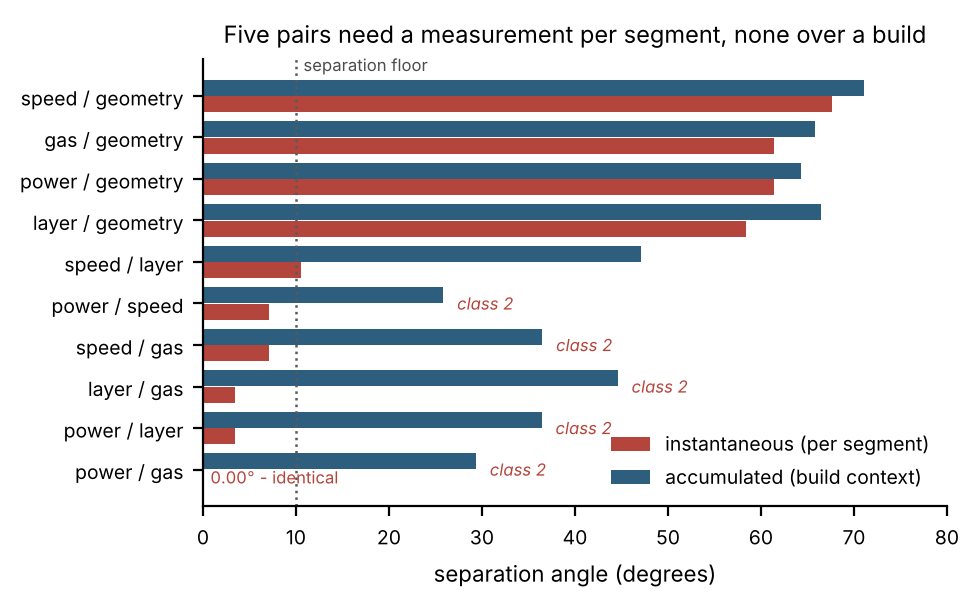
\includegraphics[width=0.80\linewidth]{fig6_matrix.png}
\caption{Diagnosability matrix for the baseline coaxial suite in both regimes.
Per-segment decisions leave five of ten pairs requiring an added measurement;
accumulated diagnosis over a build resolves all ten from existing signals.
Class 3, structurally irreducible, is empty in both regimes.}
\label{fig:matrix}
\end{figure}

\subsection{Diagnosability matrix and configuration classes}

Classifying on the enlarged observation alone places all ten pairs in class~1 for
every configuration, including a single photodiode --- true but uninformative.
The matrix is therefore reported in two regimes: \emph{instantaneous},
per-segment decisions for closed-loop control, and \emph{accumulated}, diagnosis
over a build for qualification and drift monitoring. The baseline suite gives five of ten pairs in class~1 instantaneously
and ten of ten accumulated, with \textbf{class~3 empty in both regimes}
(Fig.~\ref{fig:matrix}): nothing is structurally irreducible for this suite.

No vendor is named in Table~\ref{tab:configs}: mapping a product to a set of
observables rests on secondary literature rather than datasheets, since
detection bands are routinely withheld and published descriptions of the same
product disagree, so attaching a product name to a computed limit would assert
more than the evidence carries. Stripping the names also reveals what a
vendor-by-vendor table hides --- across five commercial systems surveyed there
are only three distinct configurations for this analysis.

\begin{table}[htbp]
\centering
\caption{Diagnosability by configuration class. Class~1 counts pairs resolvable
from existing signals; the last column is the instantaneous power/gas angle. E is
a configuration type, not a surveyed product.}
\label{tab:configs}
\small
\begin{tabular}{@{}llccc@{}}
\toprule
 & Configuration & Rank & Class 1 & power/gas \\
\midrule
A & single coaxial photodiode          & 1 & 0/10 & $0.00^\circ$ \\
B & photodiode + pool imaging          & 2 & 4/10 & $0.00^\circ$ \\
C & two photodiodes, separate bands    & 2 & 0/10 & $0.00^\circ$ \\
D & research reference (B + pyrometry) & 3 & 5/10 & $0.00^\circ$ \\
E & C + upstream power monitoring      & 3 & 4/10 & $\mathbf{84.02^\circ}$ \\
\bottomrule
\end{tabular}
\end{table}

\textbf{No configuration built solely from melt-pool observables separates laser
power from gas degradation}, whatever its sensor count: A through D all read
$0.00^\circ$, for the reason given in Section~\ref{sec:melt}. Configuration E is
the actionable row --- a direct measurement of delivered laser power sampled
\emph{upstream} of the process zone separates the pair at $84.02^\circ$, because
such a sensor sees the laser output without the plume attenuation. One surveyed
system may belong at E rather than C, depending on whether its laser-energy
photodiode samples upstream; this could not be established from public
documentation, so it is counted conservatively as C. Note also that C performs worse than B despite both having two
observables: two bands of the same emitted light are near-redundant, whereas a
geometric measurement adds a direction.

\subsection{What an added measurement would buy}
\label{sec:added}

The sensors most likely to help --- plume sensing for the gas fault, powder-bed
or recoater sensing for the layer fault \cite{Liu2022,Bugatti2022} --- cannot be
simulated by a model with neither a plume nor a powder layer. What such a sensor
\emph{measures} can be: a unit row on fault $k$ with a given relative noise, the
idealised best case for any instrument aimed at that cause.

A direct gas measurement clears power/gas, speed/gas and layer/gas; a direct
geometry measurement clears nothing and leaves the rank at 3, geometry being
already separated at 58--$68^\circ$. \textbf{Precision is almost irrelevant}:
sweeping the added sensor's relative noise from 50\,\% to 0.2\,\% leaves the worst
pair at $3.46^\circ$ and the cleared count at 8 of 10 throughout, because adding
a row in a new direction changes the rank while making an existing row quieter
does not. A crude measurement of the right cause beats a precise measurement of
the wrong one.

The comparison that matters follows. \textbf{Build context outperforms two
idealised, perfect direct measurements of the causes themselves}: gas and layer sensors together give rank 5 but a worst pair of
$7.12^\circ$, condition number 546 and nine of ten pairs cleared, against
$25.83^\circ$, 30 and ten of ten for build context at no hardware cost. Neither
added sensor says anything about power versus speed, and that pair is exactly
what spatial context resolves.

Among melt-pool observables the most valuable addition is free. Reporting the
camera's two axes separately rather than as an area is worth
\textbf{+13.40$^\circ$} on the binding pair, raising power/speed from
$25.83^\circ$ to $39.23^\circ$ and the overall worst pair to $29.34^\circ$,
whereas a short-wave infrared photodiode ($-0.08^\circ$) and a wide-band
pyrometer ($-0.13^\circ$) are worth nothing. The mechanism is the validation
result above: length carries 2.5$\times$ the variation of width and depth at
constant energy density, and an area multiplies the least informative dimension
by the most informative one.

%% ===========================================================================
\section{Discussion}
%% ===========================================================================

\subsection{Relation to reported monitoring performance}

The premise that predicted limits could be compared against reported accuracies
turns out to be mostly unrealisable, and the reason is itself the result. Of 18
works extracted, 12 classify outcomes, about which this analysis makes no
prediction: a melt pool deeper than the layer will fuse whatever made it deep. No
published work attempts to separate power from gas, or layer from power --- the
pairs identified here as confounded. That is absence of evidence rather than
evidence of absence, but no published result contradicts the predicted limits.

Where comparison is possible it is consistent. Two independent groups report the
lumped group this analysis identifies as what survives confounding: RAISE-LPBF
ranks on linear power density as a target in its own right \cite{Blanc2024}, and
parameter estimation from melt pool imagery predicts energy density class
\cite{kNN2025}. One quantitative comparison remains available and should be made
before any strong claim of model fidelity. Reijonen reports the photodiode
response to scan speed as a power law $y=ax^{-b}$ \cite{Reijonen2024}, whose
relative sensitivity is exactly $-b$ and so is directly comparable to the
Jacobian entry here, $-0.483$; the same work reports the power response as
approximately linear where the entry here, $+1.518$, is superlinear. Whether
these agree is a decisive test of the forward model.

\subsection{A design rule}

The failed and successful candidates differ by a criterion that can be stated
generally: \emph{a sensor added to break a confound must observe upstream of the
shared channel; a sensor reading the melt pool adds a row, not a direction.} This
explains why two photodiodes in different bands (C) buy nothing while an upstream
power monitor (E) buys $84^\circ$, and why plume and powder-bed sensing are the
right classes for the gas and layer faults.  Before buying an instrument, extract more
independent directions from those already fitted.

\subsection{Limitations}
\label{sec:limits}

The thermal model is a conduction solution with an analytic keyhole patch: it
partial-passes the Guo validation, absolute magnitudes are not claimed, and the
fitted parameters sit at their bounds. The absorptivity, conductivity and heat
capacity correlations of 0.93--0.96 reported during Bayesian calibration of the
same model family \cite{Hon2021} are the same pathology this paper studies,
appearing in its own calibration. One coupling remains an unmeasured estimate,
and no benchmark dataset with deliberately induced machine faults exists against
which to calibrate any of them, so each is defended by sweeping rather than by
argument.

Three modelling choices make the instantaneous case \emph{more} confounded than
reality, and so inflate the gap by which the contribution is measured. Defining
the gas fault as pure optical depth omits a convective channel a real gas fault
would have. Treating plume attenuation as independent of power and speed is what
makes the power/gas degeneracy exact, whereas the photodiode response to gas flow
is reported to depend interactively on the other parameters
\cite{Reijonen2024}, and reduced gas flow causes loss of penetration through
plume obstruction \cite{Reijonen2020}. Modelling upstream power monitoring as a
melt-pool-derived signal is likewise pessimistic.
\textbf{The reported $0.00^\circ$ should be read as an upper bound on the
instantaneous confounding.} The rank limit is unaffected, deriving from channel
counting rather than from the form of this coupling.

The modulation profiles are the largest remaining exposure. One is supported by
benchmark measurement, but by a measurement organised differently from the
regressor used here; the others are asserted. The contrast and permutation sweeps
are the defence, and a partial one: they establish how much a wrong profile
costs, not that the assumed profiles are right. Finally, the five fault
magnitudes are physical quantities but not on a common severity scale, so
comparisons \emph{across pairs at fixed magnitude} are not meaningful. All
results are diagnosability statements --- what a suite can distinguish in
principle, at a given relative noise, under a given forward model --- not that
any algorithm achieves it.

%% ===========================================================================
\section{Conclusions}
%% ===========================================================================

Laser power deviation and shielding gas degradation produce identical melt pools
in this model, confounded at $0.00^\circ$ by algebra rather than by noise, so no
instrument reading the melt pool separates them from a single instant. The
binding limit is the melt pool, which offers four physical channels, not the
instrumentation: seven observables raise the attainable rank only from 3 to 4, at
a condition number of $2.3\times10^{5}$, leaving the worst pair at $0.00^\circ$.

The structure already present in a build dissolves the limit at no hardware cost
--- rank 3 $\rightarrow$ 5, worst pair $0.00^\circ \rightarrow 25.83^\circ$ ---
surviving at 40\,\% of the asserted profile strength and at fault magnitudes from
0.2\,\% to 20\,\%, with a shared-profile control reproducing the instantaneous
result exactly and so confirming the mechanism. That free method outperforms two
idealised direct measurements of the causes themselves, because neither addresses
power versus speed, and it requires only that the recoater and gas signatures,
and the speed and gas signatures, vary differently across a build.

No configuration built from melt-pool observables alone separates power from gas
instantaneously; an upstream measurement of delivered laser power does, at
$84^\circ$, and that is the recommendation for real-time control. Among
melt-pool observables the most valuable addition is free --- reporting the
camera's two axes separately is worth $+13.40^\circ$ on the binding pair, while
two further instruments are worth nothing. Nothing is structurally irreducible
for this suite: post-build diagnosis needs no new hardware, real-time per-segment
isolation does, and crude sensing of the right cause suffices. The method needs
only a forward model and a sensor description, and answers at specification time
a question otherwise settled after the hardware is bought.

%% ===========================================================================
%% TODO before submission: add funding and acknowledgements section if required.

%% ===========================================================================
\begin{thebibliography}{99}
\footnotesize\raggedright
\setlength{\itemsep}{0pt}\setlength{\parskip}{0pt}

\bibitem{Krysander2008}
M. Krysander, E. Frisk, Sensor placement for fault diagnosis, IEEE Trans. Syst. Man Cybern. A 38 (6) (2008)
1398--1410.

\bibitem{Frisk2017}
E. Frisk, M. Krysander, D. Jung, A toolbox for analysis and design of model
based diagnosis systems for large scale models, IFAC-PapersOnLine (2017).
doi:10.1016/j.ifacol.2017.08.504.

\bibitem{Scime2019}
L. Scime, J. Beuth, Using machine learning to identify in-situ melt pool
signatures indicative of flaw formation in a laser powder bed fusion additive
manufacturing process, Addit. Manuf. 25 (2019) 151--165.

\bibitem{Raj2023}
A. Raj, Y. Huang, R. Stegman, et al., Modeling spatial variations in co-axial melt pool monitoring signals in laser
powder bed fusion, J. Manuf. Process. 89 (2023) 24--38.

\bibitem{Blanc2024}
C. Blanc, A. Ahar, K. De Grave, Reference dataset and benchmark for
reconstructing laser parameters from on-axis video in powder bed fusion of bulk
stainless steel, arXiv preprint arXiv:2409.12475 (2024).

\bibitem{Reijonen2024}
J. Reijonen, Effect of laser parameters and shielding gas flow on co-axial
photodiode-based melt pool monitoring signals in laser powder bed fusion,
Addit. Manuf. Lett. 11 (2024) 100244.

\bibitem{Reijonen2020}
J. Reijonen, A. Revuelta, T. Riipinen, et al., On the effect
of shielding gas flow on porosity and melt pool geometry in laser powder bed
fusion additive manufacturing, Addit. Manuf. 32 (2020) 101030.

\bibitem{Liu2022}
T. Liu, C. S. Lough, H. Sehhat, et al., In-situ infrared thermographic inspection for local powder layer
thickness measurement in laser powder bed fusion, Addit. Manuf. 55
(2022) 102873.

\bibitem{Bugatti2022}
M. Bugatti, B. M. Colosimo, The intelligent recoater: A new solution for in-situ
monitoring of geometric and surface defects in powder bed fusion, Addit. Manuf. Lett. 3 (2022) 100048.

\bibitem{kNN2025}
Estimation of laser powder bed fusion process parameters from melt pool images
using k-nearest neighbours, Int. J. Adv. Manuf. Technol. (2025). doi:10.1007/s00170-025-15591-y.

\bibitem{Guo2019}
Q. Guo, C. Zhao, M. Qu, et al., In-situ
characterization and quantification of melt pool variation under constant input
energy density in laser powder bed fusion additive manufacturing process,
Addit. Manuf. 28 (2019) 600--609.

\bibitem{Weaver2024}
J. S. Weaver, D. Deisenroth, S. Mekhontsev, et al., Cross-sectional melt pool geometry of laser scanned tracks and pads on nickel
alloy 718 for the 2022 additive manufacturing benchmark challenges, Integr. Mater. Manuf. Innov. 13 (2024) 363--379.

\bibitem{Hon2021}
P. Honarmandi, R. Seede, L. Xue, et al., A rigorous test and improvement of the
Eagar-Tsai model for melt pool characteristics in laser powder bed fusion
additive manufacturing, Addit. Manuf. 47 (2021) 102300.

\bibitem{Trapp2017}
J. Trapp, A. M. Rubenchik, G. Guss, M. J. Matthews, In situ absorptivity
measurements of metallic powders during laser powder-bed fusion additive
manufacturing, Appl. Mater. Today (2017).
doi:10.1016/j.apmt.2017.08.006.

\end{thebibliography}

\end{document}
